\documentclass[11pt,a4paper]{article}
\usepackage[utf8]{inputenc}
\usepackage[T1]{fontenc}
\usepackage{charter}
\usepackage{amsmath,amssymb,amsthm}
\usepackage[margin=0.68in,top=0.62in,bottom=0.62in]{geometry}
\usepackage{graphicx,booktabs,tabularx,array,enumitem,hyperref,xcolor,fancyhdr,microtype,caption,float,lastpage}
\definecolor{primary}{RGB}{27,79,114}
\definecolor{graytext}{RGB}{80,80,80}
\hypersetup{colorlinks=true,linkcolor=primary,citecolor=primary,urlcolor=primary}
\setlength{\parskip}{3pt plus 1pt minus 1pt}
\setlength{\parindent}{0pt}
\setlist{nosep,leftmargin=*}
\setlength{\tabcolsep}{3.2pt}
\renewcommand{\arraystretch}{1.04}
\setlength{\headheight}{14pt}
\setlength{\emergencystretch}{2.5em}
\pagestyle{fancy}
\fancyhf{}
\fancyhead[L]{\fontsize{10.5}{12}\selectfont\color{graytext}2026 MCM Senior Track -- Problem B}
\fancyhead[R]{\fontsize{10.5}{12}\selectfont\color{graytext}Page \thepage\ of \pageref{LastPage}}
\fancyfoot[C]{\fontsize{10.5}{12}\selectfont\color{graytext}Capacity-valid GPU scheduling}
\renewcommand{\headrulewidth}{0.35pt}
\newcommand{\method}[1]{\texttt{#1}}
\newcommand{\takeaway}[2]{\vspace{2pt}\noindent\colorbox{primary!8}{\parbox{\dimexpr\textwidth-2\fboxsep\relax}{\vspace{2pt}\textbf{\color{primary}#1:} #2\vspace{2pt}}}\vspace{2pt}}

\begin{document}
\begin{center}
{\Large\bfseries\color{primary} Capacity-Valid Scheduling of a Heterogeneous GPU Cluster}\\[3pt]
{\large 2026 HKUST-GZ MCM Senior Track -- Problem B}\\[5pt]
\end{center}
\takeaway{Main findings}{The trace is concentrated and A10 is pressure-limited under immediate starts. On the complete A10 set, SPT-HOL gives 32.906 h mean waiting versus 34.967 h for SPT-FILL and is 1.4744 times its equal-job lower bound. Ratio placement constructs zero waiting for all 9,643 GS1 jobs in the fixed instance. For substitution, R0 is preferred for SPT-HOL at $\sigma=1$ on A10 JCT, while R-shape has the lower FCFS JCT at both tested speeds and removes 605 shape-incompatible candidates; the choice is conditional on native-pool cost and duration risk.}
\textbf{Data and validation.} We use the supplied 224,112-job trace, exact integer-second durations, six model pools, non-preemptive gang starts, and complete drain for waiting/JCT. Allocation rates use the fixed 90-day window. We independently checked original IDs and requested fields, replayed node-level CPU/GPU ledgers, verified full drain and fixed-window counts, and recomputed the published metrics from saved schedules. The seven merged V2 cases and fourteen persisted Q2 replays were already validated; this revision performs no scheduler rerun.

\section{Question 1: Workload structure and capacity pressure}
\label{sec:r1q1}
The supplied trace has 224,112 jobs on 4,278 nodes, with 10,412 GPUs and 632,636 vCPUs across six GPU models. For job $j$, $a_j$ is release time, $p_j$ duration, $W_j$ workers, and $(g_j,c_j)$ the per-worker GPU and vCPU requests. Submitted GPU work is $H_j=W_jg_jp_j$; it is a request-based quantity, not measured device utilization. The six isolated pools are summarized in Table~\ref{tab:r1pools}. The exact input hashes and the serialization comparison are in the provenance record, so the claims below use the formal-run CSV.

\begin{table}[H]\centering\caption{Six pools under the SPT-HOL full-cluster evidence. Waiting uses complete drain; allocation and completion use $[0,H)$ with $H=7,776,000$ s.}\label{tab:r1pools}\begin{tabular}{lrrrrrr}
\toprule
Pool & Jobs & GPUs & Mean wait (h) & Median/P99 (h) & GPU/CPU alloc. & $90$d done\\
\midrule
A10 &111,284&2,494&32.906&0.023/1542.181&99.922\%/17.927\%&107,002\\
A100-SXM4-80GB&80,877&3,456&0.000&0.000/0.000&62.755\%/42.032\%&80,101\\
GPU-series-1&9,643&1,558&0.434&0.000/14.492&60.779\%/34.787\%&8,213\\
GPU-series-2&13,633&976&0.016&0.000/0.045&56.931\%/37.424\%&13,606\\
H800&4,716&1,752&0.016&0.000/0.000&55.816\%/52.193\%&4,705\\
A800-SXM4-80GB&3,959&176&0.115&0.000/4.390&57.311\%/49.493\%&3,943\\
\bottomrule
\end{tabular}\end{table}

\begin{figure}[H]\centering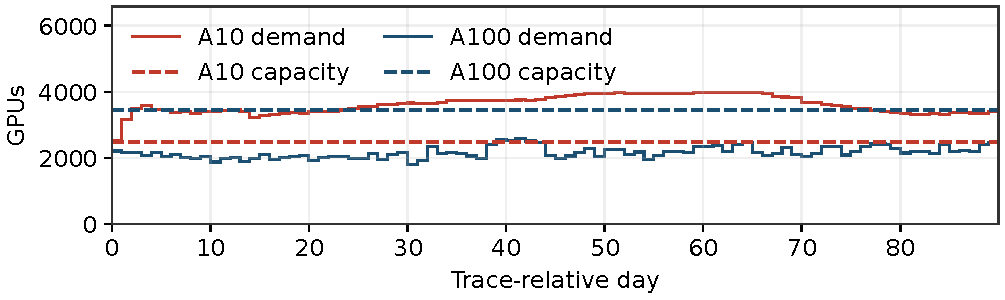
\includegraphics[width=\linewidth]{r1_figures/fig1_demand.pdf}\caption{Exact daily-bin overlap of the immediate-start counterfactual and physical GPU capacity. This is demand/capacity, not simulated allocation. The A10 mean is 3,614.54 GPUs against 2,494 capacity and its peak is 4,103; A100 demand stays below its 3,456-GPU capacity.}\label{fig:r1demand}\end{figure}

The workload is concentrated: GPU-work Gini is 0.9522, the top 1\% (2,241 jobs) contributes 43.30\%, and the top 5\% (11,205 jobs) contributes 87.68\%. Median duration is 1,330 s, the 95th percentile is 309.09 h, and the maximum is about 184 days. There are 3,512 jobs at trace time zero; without a calendar origin, their position is reported as a trace-origin batch rather than a weekday effect. The exposure-corrected relative 24-hour profile peaks at phase hour 16 and is lowest at hour 4 (ratio 2.29); this is a relative phase diagnostic, not a timezone claim.

The shape is also strongly single-worker: 90.95\% of jobs use one worker, 78.42\% use one GPU per worker, and the means are 1.539 workers and 2.003 GPUs per worker. Daily arrivals are nonstationary at the trace scale: the first day contains 8,509 jobs, day 1 contains 5,525, and the minimum is 965 jobs on day 63. These counts describe the observed window and do not identify a calendar effect or a particular arrival process.

\begin{figure}[H]\centering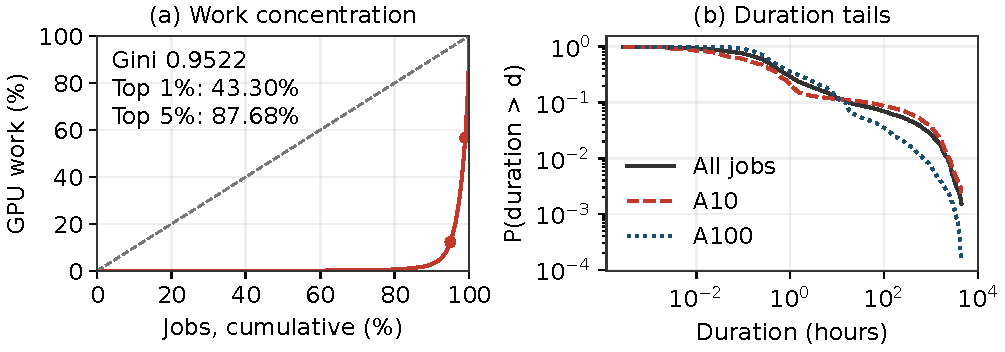
\includegraphics[width=\linewidth]{r1_figures/fig1_data_patterns.pdf}\caption{Two high-information views of the formal data: cumulative GPU-work concentration and strict duration tails.}\label{fig:r1patterns}\end{figure}

For model $m$, with exact Q1 observation window $T=7,775,878$ s, the lifetime-work ratios are
\begin{equation}
\rho_m^{GPU}=\frac{\sum_{j\in\mathcal J_m}W_jg_jp_j}{T\sum_{i\in\mathcal I_m}G_i},\qquad
\rho_m^{CPU}=\frac{\sum_{j\in\mathcal J_m}W_jc_jp_j}{T\sum_{i\in\mathcal I_m}C_i}.
\end{equation}
A10 has $\rho^{GPU}=2.064$ (Table~\ref{tab:r1pools} reports the corresponding pool work context), while GPU-series-1 has a shape mismatch: 2,478 jobs (25.70\% of that pool, 78.07\% of its work) exceed the 24-vCPU/GPU ratio of its 8-GPU, 192-vCPU nodes. The 24-, 48-, 128- and 192-vCPU/GPU configurations contain 77, 10, 1 and 901 nodes respectively. This motivates node-level gang checks; it does not identify a unique bottleneck policy.

Two lower bounds are retained with their objectives. The GPU-work weighted A10 waiting bound is 560.521 h and weights job $j$ by $H_j$. The Q2 job-count bound is 22.3179305700 h and weights every job equally. Neither is an allocation rate, an OPT value, or a guarantee after substitution changes capacity or duration.

\section{Question 2: Capacity-valid scheduling}
\label{sec:r1q2}
\subsection{Contract and Algorithm 1}
Each GPU model is simulated as its own pool. A job starts at $s_j\ge a_j$, completes at $f_j=s_j+p_j$, and all $W_j$ workers start together. At a proposed start time, a placement $x_{ji}$ is admitted only if the \emph{pre-start} residual capacities satisfy
\begin{equation}
 g_jx_{ji}\le G_i^{free}(t),\qquad c_jx_{ji}\le C_i^{free}(t),\qquad \sum_i x_{ji}=W_j.
\end{equation}
The resulting full-time model is instead the active-job constraint $\sum_{j:s_j\le t<f_j}g_jx_{ji}\le G_i^{cap}$ and its CPU analogue. Thus a single job's check against residual capacity is not written as a whole-cluster dynamic constraint. Durations are exact integer seconds; the gang commit is atomic, non-preemptive and non-migrating.

\takeaway{Algorithm 1 (SPT-HOL)}{For each model pool, insert only arrived jobs into a shortest-processing-time heap keyed by $(p_j,a_j,\mathrm{id}_j)$. Examine the heap head. If it is infeasible on the current residual nodes, stop dispatching this pool at this timestamp (head-of-line blocking). If feasible, scan nodes in the selected placement order, verify every worker slot's GPU and CPU residual, then commit all workers atomically and schedule one completion event. For GPU-series-1 only, GS1 uses a CPU/GPU-ratio node order before the same full slot check; every other pool uses ascending-ID first fit. Advance to the next arrival or completion and repeat.}

The historical program label \texttt{SJF-HOL} means this same method; the paper name is uniformly \method{SPT-HOL}. \method{SPT-FILL} uses the same key but may inspect later feasible jobs under the fixed $K=200$ bypass budget. A heap insertion or removal costs $O(\log n)$; a dispatch also scans candidate nodes and worker slots, and ratio placement orders the candidate nodes by shape. Multiple starts at one timestamp can repeat these scans, so an $O(\log n)$ event claim would be incomplete. The seven integrated cases used the same 224,112 IDs and passed independent route, physical and metric checks; their total wall time was 520.74 s with a 512.75 MiB maximum observed RSS.

The usual simultaneous-release explanation has explicit conditions: a continuously backlogged single-worker queue, zero free slots immediately after each dispatch, homogeneous single-GPU nodes, and a fill rule that is not truncated before the queue head is considered. Under these conditions, a dispatch can release capacity only when the preceding job completes, so zero waiting is a mechanism explanation. With the tested $K$ bypass limit, this remains a compatible interpretation of the observed trace rather than a theorem for all arrival patterns or bypass settings.

\subsection{A count lower bound and exact accounting}
For the complete A10 set let $C=2,494$, $G_j=W_jg_j$, $Z(t)=\{j:a_j\le t<a_j+p_j\}$, and let $q(t)$ be the minimum number of jobs removed from $Z(t)$ so that the remaining GPU width is at most $C$. For a schedule, let $S(t)=\{j:s_j\le t<f_j\}$ and $A(t)=S(t)\cap Z(t)$. At any $t$, at least $q(t)$ jobs in $Z(t)$ cannot be simultaneously active, hence $|Z(t)\setminus A(t)|\ge q(t)$. Integrating and using the waiting identity gives
\begin{equation}
\sum_j\min(\omega_j,p_j)=\int |Z(t)\setminus A(t)|\,dt\ge\int q(t)\,dt,
\qquad \sum_j\omega_j\ge\int q(t)\,dt,
\end{equation}
so $L_{count}=(3600N)^{-1}\int q(t)dt=22.3179305700$ h is a lower bound on equal-weight mean waiting. For the observed schedule,
\begin{equation}
\omega_j=\min(\omega_j,p_j)+\max(\omega_j-p_j,0).
\end{equation}
The exact full-A10 SPT-HOL JSON accounting is
\begin{center}
\texttt{\{capacity\_lb:22.3179305700, within\_window\_gap:8.3361103922, beyond\_duration:2.2524130728, mean:32.9064540350\}}.
\end{center}
These are accounting terms around a relaxation, not causal shares or an exact OPT gap. The conservative certificates $\bar\omega/L$ are 1.4744 for ordinary job mean and 1.2090 for GPU-work-weighted mean (the latter compares 677.689933 h with the 560.521368 h weighted bound); they are for this fixed instance and different objectives.

\subsection{Complete A10 and GS1 results}
On all 111,284 A10 jobs, SPT-HOL has mean/P95/P99/max waiting $32.906/11.087/1542.181/3017.288$ h, mean JCT 132.676 h and 107,002 completions by 90 days.

SPT-FILL has $34.967/15.130/1575.462/3015.311$ h, mean JCT 134.737 h and 106,802 completions. The paired mean difference is $-2.060576$ h (55,266 improved, 50,575 worsened, 5,443 unchanged), so this is a trace-specific mean result rather than dominance. The GPU-work-weighted means are 677.689933 h (SPT-HOL) and 677.495535 h (SPT-FILL), illustrating the objective change.

The complete full-cluster SPT-HOL summary is Table~\ref{tab:r1pools}. It keeps pool-level allocation rates and completion counts separate from complete-drain waiting. We do not construct a cluster quantile by concatenating pool quantiles.

For the fixed GS1 pool, the corrected ratio placement is a constructive zero-wait schedule: both FCFS and SPT-HOL have 9,643/9,643 zero-wait jobs and mean waiting 0 h, while FF-id gives 0.029188 h (FCFS) and 0.434277 h (SPT-HOL). Since mean waiting is nonnegative, 0 is the optimum for this fixed GS1 instance. The ratio rule is not generalized to other heterogeneous pools.

\subsection{Second-round policy evidence}
The verified 65,536-job prefix remains a separate evidence tier. On the full A10 trace, the second-round HEAD-TIME case changes mean waiting from 32.906454 to 32.923817 h, P99 from 1542.181042 to 1541.586592 h, and maximum from 3017.288056 to 3017.727778 h; its higher cost is not hidden by a single tail statistic. The K/timer and HEAD-TIME results support a bounded mechanism interpretation, not starvation freedom or a general performance theorem. The urgent policies remain prefix-only and are not promoted to the complete-trace recommendation.

\section{Question 3: Fixed-split cross-GPU substitution}
\label{sec:r1q3}
\subsection{Model and two versions of the route rule}
A job has native model $n_j$, actual model $m_j$, duration $p_j$, workers $W_j$, and per-worker requests $(g_j,c_j)$. For the sole assumed foreign edge A10$\to$A100-SXM4-80GB, $p'_j=\sigma p_j$; compatibility and $\sigma$ are scenario assumptions, not measured hardware facts. All workers start together on physical nodes, with no migration or preemption, and every start passes the same CPU/GPU slot check.

V1/S1--S5 are the historical fixed-split sensitivity runs: M0 is model isolated, and R0 (called S0 in the historical tables) reserves 60 of 432 A100 nodes for a 10\% SHA-256-selected A10 subset. V2 C0--C4 are the complete merged-runtime cases; GS1 uses ratio placement, while other pools use FF-id. The implemented V2 substitution rule is \emph{R-shape}; only Candidate B (online completion-cost routing) remains deferred. R-shape keeps only hash-selected jobs whose CPU/GPU shape fits the donor ratio, yielding 10,604 routed and 605 shape-rejected A10 jobs. It is a fixed physical counterfactual, not a claim that a dynamic policy has been implemented.

\begin{table}[H]\centering\caption{SPT-HOL V2 substitution evidence from persisted full-cluster results. Native harm is the number of native A100 jobs with positive additional waiting relative to M0; the final column is the principal harmed A10 group relative to M0.}\label{tab:r1q3main}\begin{tabular}{lrrrrrr}
\toprule
Scenario & $\sigma$ & A10 wait (h) & A10 JCT (h) & All JCT (h) & $90$d done & Native harm / A10 harmed\\
\midrule
M0 & -- &32.906&132.676&93.353&217,570&0 / 0\\
R0 &1&20.534&120.303&87.209&217,814&0 / 49,772\\
R0 &2&25.106&134.810&94.412&217,521&0 / 56,422\\
R-shape &1&24.359&124.128&89.108&217,801&0 / 46,803\\
R-shape &2&24.359&129.671&91.860&217,613&0 / 55,465\\
\bottomrule
\end{tabular}\end{table}

For FCFS, R0 $\sigma=1$ gives A10 mean wait 587.875 h and all-job mean JCT 368.910 h; R-shape gives 656.356 h and 402.914 h. At $\sigma=2$, FCFS R0 has A10 mean JCT 831.456 h, whereas R-shape has 761.668 h. Thus the largest-JCT comparison is favorable to R-shape at both tested speeds for the displayed policy, while R0 is better for SPT-HOL at $\sigma=1$ (A10 JCT 120.303 versus 124.128 h). These are two measured points, not an upper bound over $[1,2]$, an unknown-speed guarantee, or a unique $\sigma^*$.

\subsection{What the trade-off means}
For SPT-HOL, R0 is the more aggressive 10\% split; R-shape rejects 605 high-CPU/GPU jobs and changes the selected load. At $\sigma=1$, R0 reduces A10 wait relative to M0, while R-shape has a smaller A10 benefit but lower paired positive completion-delay mass (16,051.659 job-hours versus R0's 68,183.183 job-hours). At $\sigma=2$, common routed-job ordering is unchanged because all durations in one foreign queue are multiplied by the same $\sigma$; re-simulation is still required because completion/release interactions change. R-shape's A10 wait is unchanged at 24.359 h between the two tested speeds, but A10 JCT rises 5.542 h and 90-day completions fall by 188.

The A100 physical allocation comparison uses one full-pool denominator of 3,456 GPUs and sums native plus foreign occupancy. For SPT-HOL, R0 $\sigma=1$ is 0.7224 (native 2,976-GPU partition 0.6276 plus foreign 480-GPU partition 0.0948); R-shape is 0.6899 at $\sigma=1$ (0.7288 native plus 0.4492 foreign) and 0.7148 at $\sigma=2$ (0.7288 plus 0.6284). A larger partition rate is not called a utilization gain by shrinking the native denominator.

\begin{figure}[H]\centering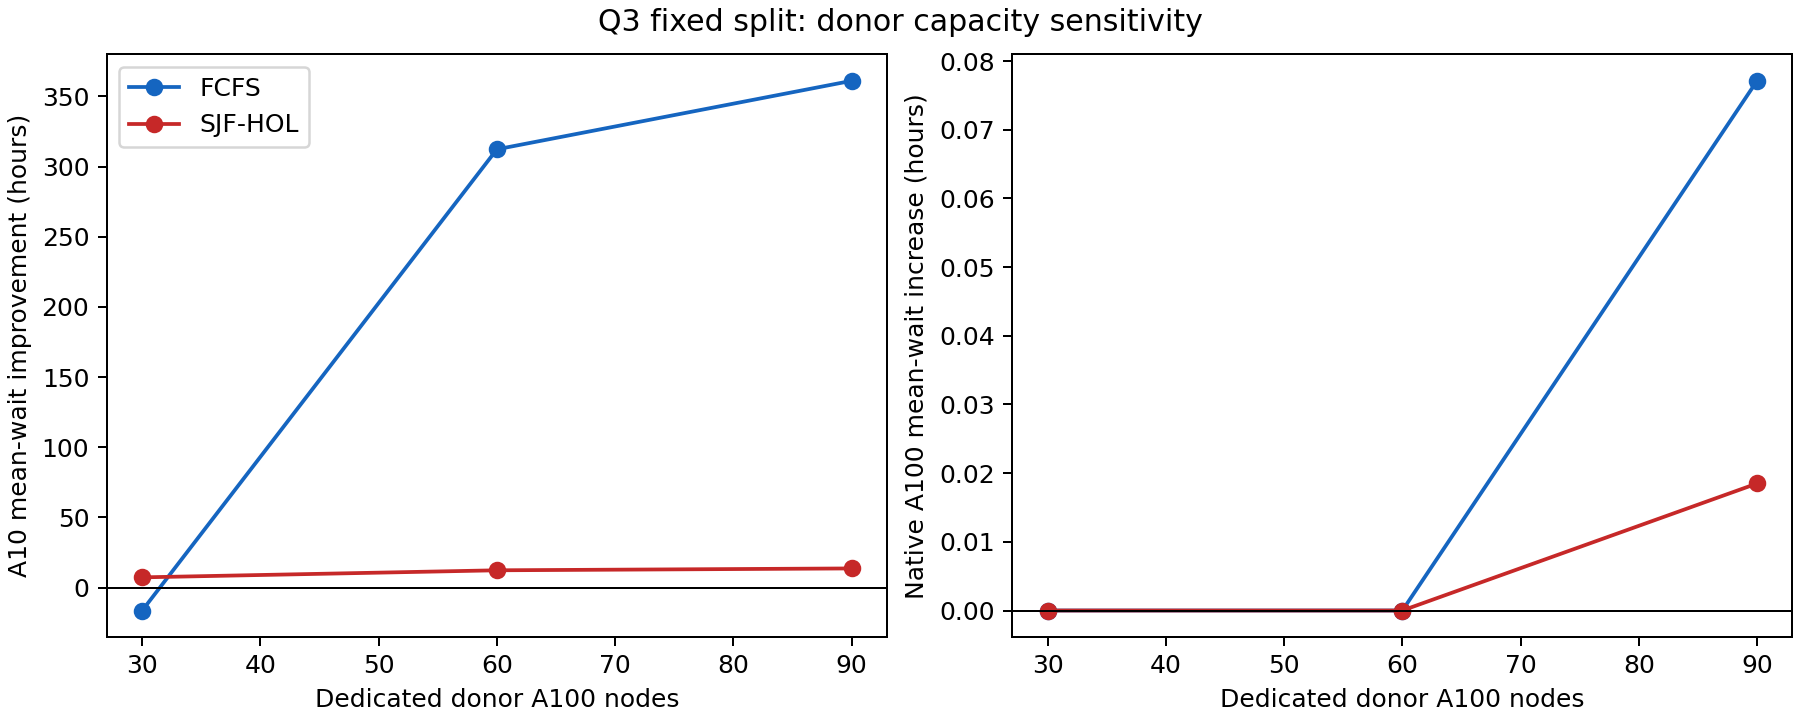
\includegraphics[width=0.86\linewidth]{figures/q3_donor_capacity_wait_tradeoff.png}\caption{V1/S1--S5 donor-capacity sensitivity. The left panel is A10 mean-wait change; the right panel is native A100 mean-wait change, with separate scales.}\label{fig:r1q3tradeoff}\end{figure}

The historical sensitivity retains its negative cases: at 60 donors, 20\% routing raises FCFS A10 mean wait to 1,010.136 h and its maximum to 5,445.367 h; 30 donors at 10\% gives 916.407 h, worse than M0. For the 90-donor case, SPT-HOL native A100 has 2,150 positive-delay jobs, mean additional wait 0.018492 h over all 80,877 native jobs, and harmed-subgroup mean 0.695606 h. These finite paired results expose the management choice between A10 relief, native harm, tail, and completion count.

A financial extension is optional rather than a second experiment. If a tenant values completion time at $v$ per hour and pays $P$, voluntary substitution requires payment reduction at least $v$ times the completion-time increase. No price, participation rate, revenue, or profitability is inferred here. The online Candidate B rule is recorded as future work, and no new 480-job batch policy or borrowed threshold is introduced.


\section{Conclusion, limits, and provenance}
The three questions answer different decisions. Q1 separates submitted work, immediate-start demand, and simulated allocation. Q2 provides a capacity-valid SPT-HOL contract, a count lower bound, a zero-wait GS1 construction, and complete-A10 tail and cost evidence. Q3 compares fixed physical partitions and speed assumptions while retaining native harm and duration sensitivity. These are finite trace results: allocation is request occupancy, GPU-hours across models are not interchangeable hardware or monetary units, and no heuristic optimality, speed guarantee, or dynamic substitution policy is claimed. Candidate B remains deferred. The original job ZIP bytes are not in this repository; the available historical-hash file is parsed-equivalent to the formal-run CSV but has different BOM/newline serialization, as recorded in the supplement provenance.

\section*{References}
\begin{enumerate}
\item HKUST-GZ MCM 2026 Senior Track, Problem B, repository copy (official question PDF; hash in the source index).
\item Graham, R. L. (1966), ``Bounds on multiprocessing timing anomalies,'' \emph{SIAM Journal on Applied Mathematics}, 14(2), 416--429. Used only as scheduling background; the reported lower bound is derived for this trace.
\item Feitelson, D. G. (2015), \emph{Workload Modeling for Computer Systems Performance Evaluation}. Used for workload-trace terminology and the distinction between demand and allocation.
\item SchedMD, ``Backfill scheduling'' documentation. Used to distinguish a feasible-fill bypass from SPT head-of-line blocking.
\end{enumerate}

\section*{Use of AI Tools}
ChatGPT and OpenAI Codex were used for research discussion, source and data inspection, mathematical-notation assistance, read-only post-processing, plot generation, code and evidence cross-review, and English drafting/typesetting. Claude was used in the earlier research record for independent prototype analysis and cross-review; its archive was preserved and its unverified prototype numbers were not used as formal results. The formal scheduler runs, saved-ledger replays, metric recomputation, and final submission decisions remain team responsibilities. The team must complete the human review and confirm the final identity and wording before submission.
\end{document}
